% Revision 4 -- generalisation over the problem space (answers "the considered scenario is too simple").
% Numbers: paper_rev4/generated/{tab_sweep,tab_sweep_pattern}.tex, sweep_macros.tex, sweep_paired.csv,
% sweep_defendable.csv, sweep_family.csv; data results/sweep/*.csv (sim/sweep.py, sim/generic.py).
\subsection{Generalisation: a randomised sweep over the problem space}\label{sec:sweep}

S1--S14 are single points of the scenario space of Sec.~\ref{sec:formulation}. To test whether the
conclusions drawn from them carry over, we drew 2{,}000 instances at random from the ranges of
Table~\ref{tab:scenario_space} (\texttt{sim/generic.py}): the eight real topologies or a Waxman or
Barab\'asi--Albert graph of 15--40 nodes with uniform or mixed (10/40/100\,Mbps) capacities; a
gravity-model demand of 10--60 flows scaled so that static routing loads the busiest link to
U[0.2,\,0.6]; one to three attacked links, each with one to five bots; an attack intensity $\alpha$
(the targets' offered load over capacity) drawn from U[0.9,\,1.6]; and one of four behaviours ---
constant, pulsing (period 4 or 8\,s, duty $\tfrac13$, $\tfrac12$ or $\tfrac23$), timed bursts, or
rolling re-targeting at the link the victims share under the current routing. 55 instances, all
Waxman graphs, had no attackable link (every fastest link was a bridge or crossed by no host pair) and
were dropped; the remaining \sweepN{} instances (11--50 nodes, 14--99 links) were each run with seven
systems, \sweepRuns{} runs in total. All systems see the same instance (it is seeded by its id) and the
same candidate-path limit (the 20 lowest-latency paths within the hop limit). For every instance we
also solved (\ref{eq:phistar}), which gives $\Phi^\star$, defendability and the remaining excess of each
system. Under the rolling attack the demand depends on the routing, so $\Phi^\star$ is solved for each
system's own demand; when a system's reroutes provoke an attack whose $\Phi^\star$ is already at least
$\Phi_{\mathrm{static}}$ (40--84 rolling instances per system), the ratio is undefined, and we count the
instance as infinitely bad if the system's $\Phi$ exceeds $\Phi_{\mathrm{static}}$ and as 1 otherwise,
rather than dropping it.

\paragraph{Defendability}
\sweepDefend\,\% of the instances are defendable ($\Phi^\star=0$). As Proposition~\ref{prop:cut}
predicts, the share falls with the attack intensity and the number of targets: from 91\,\% for one
target and $\alpha\le1.1$ to 23\,\% for three targets and $\alpha>1.3$
(\texttt{sweep\_defendable.csv}). Sparse Waxman graphs are defendable less often (42\,\%) than
Barab\'asi--Albert graphs (68\,\%) and the real topologies (64\,\%), since they have fewer disjoint
detours. In the remaining 39\,\% no controller can keep every link below $\theta$, and the right
question is how close to $\Phi^\star$ a system gets, which the remaining excess measures.

\IfFileExists{generated/tab_sweep.tex}{\begin{table}[t]\centering\scriptsize
\caption{Randomised sweep over the problem space (1945 instances, Sec.~\ref{sec:sweep}). Remaining excess: $(\Phi-\Phi^\star)/(\Phi_{\mathrm{static}}-\Phi^\star)$, 0 = optimal, 1 = no better than static routing (median [IQR]); $>$static: share of instances with a remaining excess above 1. Relieved: share of defendable instances ($\Phi^\star=0$) in which no target stayed above $\theta$ for more than 10\,s. Victim loss and moves (flow reroutes) are means over all instances.}
\label{tab:sweep}
\setlength{\tabcolsep}{3pt}
\begin{tabular}{lrrrrr}
\toprule
System & remaining excess & $>$static & relieved & victim loss \% & moves\\
\midrule
Static & 1.00 [1.00, 1.00] & 0\% & 0\% & 16.00 & 0.0\\
k-MP & 0.49 [0.11, 4.39] & 32\% & 51\% & 9.67 & 0.0\\
Reactive & 1.44 [0.95, 4.75] & 71\% & 30\% & 18.43 & 359.3\\
TE-$\Phi$ & 0.09 [0.03, 0.13] & 3\% & 81\% & 4.17 & 10.4\\
RSDN & 0.70 [0.38, 0.99] & 8\% & 26\% & 7.34 & 6.8\\
RSDN-v2 & 0.52 [0.30, 0.98] & 9\% & 47\% & 6.83 & 8.0\\
RSDN-v3 & 0.40 [0.20, 0.78] & 9\% & 63\% & 5.61 & 8.9\\
\bottomrule
\end{tabular}
\end{table}}{}

\paragraph{Overall ranking}
Table~\ref{tab:sweep} and Fig.~\ref{fig:sweep_cdf} rank the systems over the whole space. The ordering
of the hand-made scenarios largely carries over, with one exception: $k$-MP, behind ResilientSDN in
S1--S14 (45 against 35\,s above $\theta$), is ahead of it here. TE-$\Phi$ comes closest to the optimum (median
remaining excess \sweepGaptelpexcess), followed by ResilientSDN-v3 (\sweepGapresilientsdnvThree),
$k$-MP (\sweepGapmpksp), v2 (\sweepGapresilientsdnvTwo), ResilientSDN (\sweepGapresilientsdn) and
simple reactive rerouting (\sweepGapsimplereactive, worse than static routing in 71\,\% of the
instances). $k$-MP and v2 have similar medians but different distributions: static three-way
splitting is worse than not reacting in 32\,\% of the instances (upper quartile 4.39), spread evenly
over all attack patterns, while the ResilientSDN variants are worse than static routing in 8--9\,\%,
almost all of them rolling attacks (below).
Paired over instances (Wilcoxon, Holm-corrected over the twelve comparisons with ResilientSDN), v3
has lower $\Phi$ than ResilientSDN in 1{,}277 instances, equal in 443 and higher in 225
($p<10^{-100}$, rank-biserial $-0.69$), and lowers the mean victim loss from 7.34 to 5.61\,\% (95\,\%
CI of the difference $[-1.99,-1.47]$ points); TE-$\Phi$ has lower $\Phi$ in 1{,}894 of the
1{,}945 instances. The remaining excess is a relative measure; in absolute terms, means are dominated
by a few instances with very large excess, which is why the table reports medians.

\begin{figure}[t]\centering
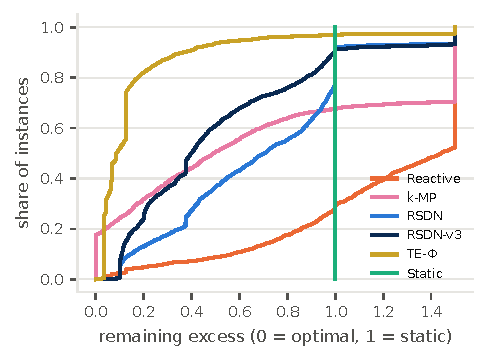
\includegraphics[width=\columnwidth]{figures/sweep_cdf}
\caption{Distribution of the remaining excess over the \sweepN{} sweep instances (0 = instance
optimum $\Phi^\star$, 1 = static routing; clipped at 1.5).}\label{fig:sweep_cdf}
\end{figure}

\IfFileExists{generated/tab_sweep_pattern.tex}{\begin{table}[t]\centering\scriptsize
\caption{Sweep by attack pattern: median remaining excess / share of defendable instances relieved (definitions as in Table~\ref{tab:sweep}). Instances per pattern: constant 519, timed 452, pulse 482, rolling 492.}
\label{tab:sweep_pattern}
\setlength{\tabcolsep}{3pt}
\begin{tabular}{lrrrr}
\toprule
System & constant & timed & pulse & rolling\\
\midrule
k-MP & 0.45 / 49\% & 0.45 / 59\% & 0.50 / 49\% & 0.54 / 47\%\\
Reactive & 1.55 / 8\% & 1.45 / 92\% & 1.38 / 12\% & 1.39 / 3\%\\
TE-$\Phi$ & 0.03 / 89\% & 0.13 / 88\% & 0.07 / 87\% & 0.13 / 51\%\\
RSDN & 0.39 / 42\% & 0.65 / 40\% & 1.00 / 6\% & 0.67 / 8\%\\
RSDN-v2 & 0.13 / 80\% & 0.46 / 69\% & 1.00 / 12\% & 0.56 / 8\%\\
RSDN-v3 & 0.13 / 80\% & 0.46 / 69\% & 0.27 / 69\% & 0.52 / 9\%\\
\bottomrule
\end{tabular}
\end{table}}{}

\paragraph{Where the hand-made conclusions do and do not generalise}
Fig.~\ref{fig:sweep_factors} and Table~\ref{tab:sweep_pattern} break the results down by factor.
\emph{(i) Pulsing attacks.} Over 482 pulsing instances with random periods and duty cycles,
ResilientSDN and v2 have a median remaining excess of 1.00 and relieve only 6 and 12\,\% of the
defendable ones: the trend detector's deadband evasion of S7 and Proposition~\ref{prop:evasion} is
not an artefact of one period, but holds over the sampled range. The duty-cycle trigger of v3 closes
most of it (0.27, 69\,\% relieved), and is equal to v2 on constant and timed attacks.
\emph{(ii) Rolling attacks} are the hardest case for every system: even TE-$\Phi$, which re-optimises
every interval, relieves 51\,\% of the defendable instances, and the reactive systems 3--9\,\%.
They are also the only case in which ResilientSDN does worse than not reacting: all 151 instances in
which its $\Phi$ exceeds that of static routing (31\,\% of the 492 rolling instances) are rolling
attacks; TE-$\Phi$ is worse than static routing in 11\,\% of them. The attacker re-aims at the link
the rerouted victims now share, so each reroute moves the congestion instead of removing it, while
static routing gives it no reason to move; the ten largest such losses are on G\'EANT (4), Arnes (5)
and one Waxman graph. Because of these instances the \emph{mean} $\Phi$ of ResilientSDN over the
whole sweep (134.5) exceeds that of static routing (119.8); without the rolling instances it is 40.3
against 60.0. Proposition~\ref{prop:monotone} does not contradict this: it holds for the measured
rates of one interval, and a routing-aware attacker changes the rates in the next.
\emph{(iii) Topology.} All systems are further from the optimum on sparse Waxman graphs (v3: 0.58
against 0.38 on the real topologies). On the real topologies, $k$-MP (0.34) is slightly ahead of v3
(0.38); on random graphs, with mixed capacities and less path diversity, it falls behind every
ResilientSDN variant. \emph{(iv) Intensity and number of targets.} TE-$\Phi$ is first and simple
reactive last in every $\alpha$ and target-count bin of Fig.~\ref{fig:sweep_factors}, and v3 is ahead
of v2 and v2 of ResilientSDN in every bin. $k$-MP is second for $\alpha\le1.1$ and for one target, but
falls behind v3 as the attack grows (median 0.29 to 0.58 over the $\alpha$ bins, against 0.34 to 0.48
for v3); it is level with v2 for $\alpha>1.3$ and behind it for three targets (0.62 against 0.54).

\begin{figure*}[t]\centering
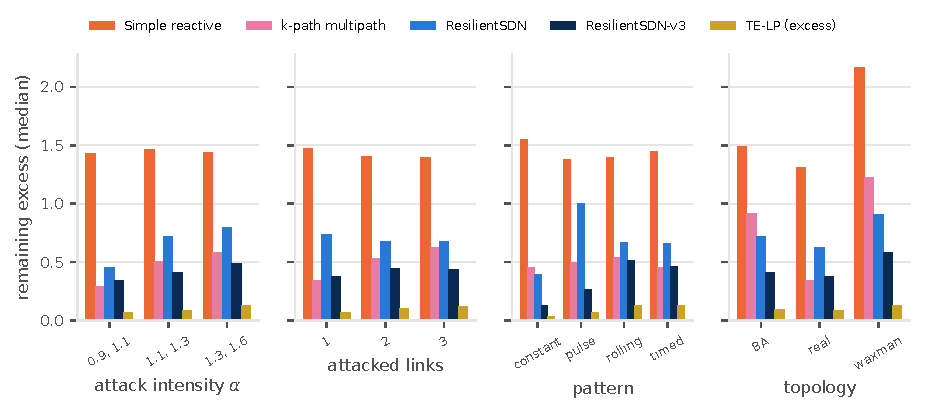
\includegraphics[width=\textwidth]{figures/sweep_factors}
\caption{Median remaining excess by attack intensity, number of attacked links, attack pattern and
topology family (\sweepN{} instances; 0 = instance optimum, 1 = static routing).}\label{fig:sweep_factors}
\end{figure*}

\paragraph{What the sweep does not cover}
The sweep runs in the flow-level simulator only, and $\Phi^\star$ is a relaxation: it splits flows
fractionally and knows the demand of each interval, so a remaining excess of 0 is a bound, not a
target an unsplittable reactive controller could reach. TE-$\Phi$ shares the fractional splitting and
the per-interval knowledge, which is why it is closest to $\Phi^\star$; it is an idealised reference,
not a deployable competitor (Sec.~\ref{sec:limits}).
